\documentclass[../main.tex]{subfiles}
\begin{document}


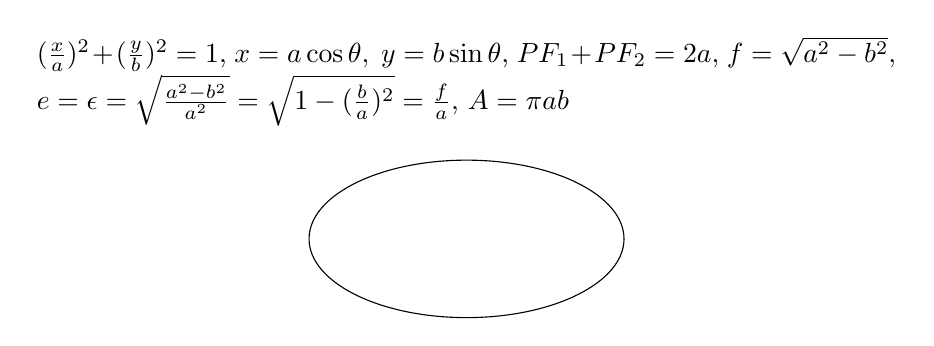
\begin{tikzpicture}

\draw ellipse (2cm and 1cm) node (o) {};
\node (prop) at (0,2) {\parbox{0.9\textwidth}{
$(\frac{x}{a})^2+(\frac{y}{b})^2=1$,
$x=a\cos{\theta},\ y=b\sin{\theta}$,
$PF_1+PF_2=2a$,
$f=\sqrt{a^2-b^2}$,
$e=\epsilon=\sqrt{\frac{a^2-b^2}{a^2}}=\sqrt{1-(\frac{b}{a})^2}=\frac{f}{a}$,
$A=\pi ab$}
};

\end{tikzpicture}

\end{document}
